%!TEX root = ../../../super_main.tex

\section{Launcher Grid Setting}
\label{sec:launcher_grid_setting}
%% Indsæt reference til usability report
We fixed a usability problem in the \launcher settings (see \figref{fig:launcher_grid_settings_old}) by changing description of grid setting and by changing the description text. The users had trouble figuring what moving the \androidinline{SeekBar} meant. Did moving the \androidinline{SeekBar} result in more or less applications in the main screen of the launcher? We changed to text to indicate the number of applications instead of the grid size. The result can be seen in \figref{fig:launcher_grid_settings_new}. 

\begin{figure}[!htbp]
        \centering
        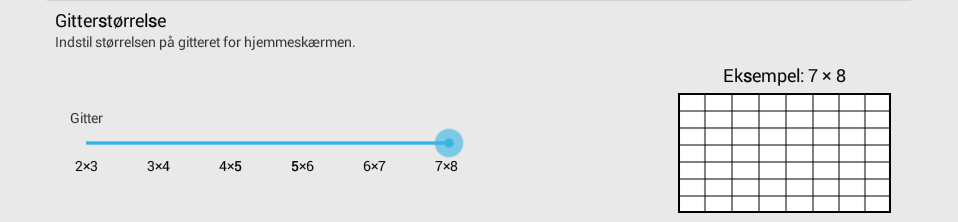
\includegraphics[width=0.75\textwidth]{sprint_four/grid_setting_before}
        \caption{Grid setting before}
        \label{fig:launcher_grid_settings_old}
\end{figure}

\begin{figure}[!htbp]
        \centering
        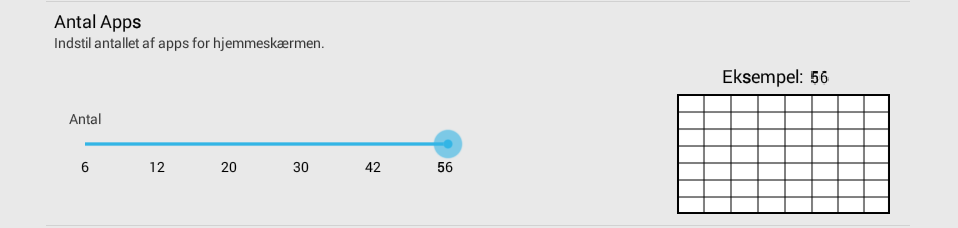
\includegraphics[width=0.75\textwidth]{sprint_four/grid_setting_after}
        \caption{Grid setting after}
        \label{fig:launcher_grid_settings_new}
\end{figure} 